\documentclass[a4paper,12pt]{report}
\usepackage{amsmath}
\usepackage{alltt, fancyvrb, url}
\usepackage{graphicx}
\usepackage[utf8]{inputenc}
\usepackage{float}
\usepackage{hyperref}
\usepackage[italian]{babel}
\usepackage{appendix}
\usepackage[italian]{cleveref}
\usepackage{xcolor}
\usepackage{microtype}
\usepackage{array}
\usepackage{adjustbox}
\usepackage{tabularx}
\usepackage{colortbl}
\usepackage{pdfpages}
\usepackage{listings}
\usepackage{booktabs}
\usepackage{longtable}
\usepackage{xltabular}
\usepackage{setspace}
\usepackage{ulem}
\usepackage{float}
\usepackage{tocloft}
\usepackage{lmodern}
\usepackage{natbib}
\usepackage{import}
\bibliographystyle{plain}



\lstdefinestyle{codeStyle}{
    basicstyle=\small\ttfamily,
    keywordstyle=\color{blue},
    commentstyle=\color{green},
    stringstyle=\color{red},
    numbers=left,
    numberstyle=\tiny\color{gray},
    frame=single,
    breaklines=true,
    tabsize=2
}
\lstdefinestyle{pseudocode}{
    basicstyle=\ttfamily,
    keywordstyle=\color{blue}\bfseries,
    commentstyle=\color{gray}\itshape,
    stringstyle=\color{red},
    morekeywords={if, else, while, for, return, function, end, begin},
    morecomment=[l]{//},
    morecomment=[s]{/*}{*/},
    morestring=[b]",
	numbers=left,
    numberstyle=\tiny\color{gray},
    frame=single,
    breaklines=true,
	tabsize=1
}

\lstset{}
\newcolumntype{C}{>{\centering\arraybackslash}X}
\newcolumntype{D}{>{\center\arraybackslash}X}

\newcommand{\speciallabel}[2]{
	% \speciallabel{<stuff>}{<label>}
  \edef\@currentlabel{#1}\label{#2}%
}

\newcommand{\tableheader}{% % il comando prende quattro argomenti
\hline % disegna una linea orizzontale
\rowcolor{red} % colora la riga di rosso
\multicolumn{1}{|C|}{\textcolor{white}{\uppercase{concetto}}} & % centra e mette in grassetto il primo argomento
\multicolumn{1}{C|}{\textcolor{white}{\uppercase{costrutto}}} & % centra e mette in grassetto il secondo argomento
\multicolumn{1}{C|}{\textcolor{white}{\uppercase{accessi}}} & % centra e mette in grassetto il terzo argomento
\multicolumn{1}{C|}{\textcolor{white}{\uppercase{tipo}}} \\ % centra e mette in grassetto il quarto argomento
\hline % disegna una linea orizzontale
}

% A new counter for the rows
\newcounter{rowcntr}[table]
\renewcommand{\therowcntr}{\table\number\numexpr\value{rowcntr}\relax}


% A new columntype to apply automatic stepping
\newcolumntype{N}{>{\refstepcounter{rowcntr}\therowcntr}l}

% Reset the rowcntr counter at each new tabular
\AtBeginEnvironment{tabular}{\setcounter{rowcntr}{0}}

\setlength{\cftbeforesecskip}{0pt} % Riduce lo spazio verticale prima delle sezioni
\setlength{\cftaftertoctitleskip}{10pt} % Riduce lo spazio verticale dopo il titolo dell'indice

\graphicspath{{../resources/img}}
\title{\Large Course: Crittografia    \\[0.5cm]
        \bf\Large Crittografia applicata alla sicurezza di tutti i giorni: Bitwarden}
\author{\large Author: Edoardo Desiderio\\ \ \\}


\date{}

\begin{document}

	\makeatletter
		\begin{titlepage}
			\begin{center}
		{ 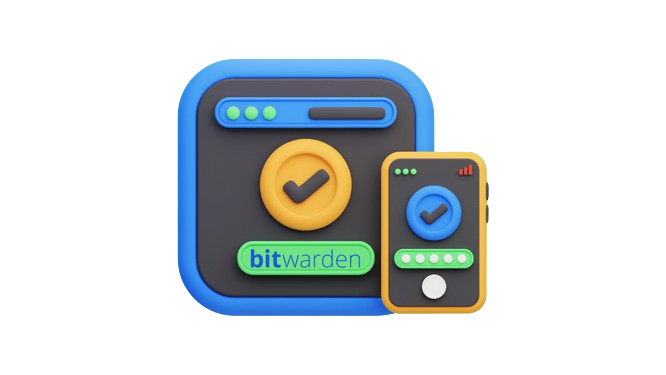
\includegraphics[width=10cm]{bitwarden-removebg-preview.png}}
		{\ \\}
			\vbox{}\vspace{2cm}
				{\@title }\\[3cm] 
				{\@author}
				{\large Instructor: \bf Prof. Luciano Margara\\ \ \\}
			\end{center}
		\end{titlepage}
	\makeatother
	\mbox{\thispagestyle{empty}}
	\titlepage
	\tableofcontents{\thispagestyle{empty}}
	\setcounter{page}{0}

	\chapter{Introduzione}
		\section{Scopo del Documento}
		La ricerca nasce dal desiderio di esplorare il ruolo della crittografia non 
		solo come strumento di protezione, ma anche come tecnologia essenziale per la
		sicurezza digitale quotidiana. Mentre spesso si parla di crittografia associata 
		a malware e ransomware, questo documento si concentra sul suo utilizzo positivo, 
		illustrando il viaggio che compie un dato per diventare sicuro.
		Attraverso il caso studio di un password manager come Bitwarden, esploreremo 
		come il dato, da semplice informazione, venga trasformato, crittografato e custodito
		in modo sicuro. L’obiettivo è fornire una visione chiara e tecnica di come i vari 
		algoritmi e processi crittografici intervengano in questa trasformazione, 
		garantendo protezione e resilienza contro attacchi esterni.
		\section{L'Uso Positivo della Crittografia} 
		La crittografia è una scienza matematica che utilizza algoritmi per
		proteggere dati sensibili, assicurare comunicazioni sicure e preservare
		l’integrità delle informazioni. Nel panorama digitale odierno, il
		“viaggio del dato” inizia con l’obiettivo di garantire riservatezza e
		sicurezza, attraversando vari processi crittografici per diventare
		inattaccabile.

		Attraverso tecnologie come gli algoritmi di crittografia simmetrica e
		asimmetrica, i dati vengono trasformati in modo che solo le parti
		autorizzate possano accedervi. In particolare, la crittografia è alla
		base di strumenti come i password manager, che consentono agli utenti di
		custodire in sicurezza le proprie credenziali.
		\section{concetti chiave per questa ricerca}
		Per comprendere appieno il viaggio che il dato compie, è fondamentale
		analizzare due principi su cui si basano gli algoritmi crittografici:
		Confusione e Diffusione. Ogni fase del processo crittografico applica
		questi concetti in modi diversi per garantire la sicurezza dei dati.

			\subsection{Confusione}
			La confusione rappresenta la capacità di nascondere la relazione tra
			il testo cifrato e la chiave crittografica. Questo è fondamentale
			per rendere difficile a un attaccante dedurre il dato originale o la
			chiave analizzando il dato cifrato. Algoritmi come DES che utilizza
			operazioni non lineari, ad esempio le S-Box, per introdurre complessità e
			imprevedibilità. In questo contesto, ogni trasformazione aumenta il
			grado di protezione, rendendo il dato sempre più difficile da
			decifrare.

			\subsection{Diffusione}
			La diffusione, invece, garantisce che una modifica anche minima nel
			dato in ingresso influenzi in maniera significativa il dato in
			uscita. Questo rende complesso per un attaccante stabilire
			corrispondenze tra il dato originale e quello cifrato. Tecniche come
			ShiftRows e MixColumns negli algoritmi AES mescolano i dati su più
			livelli, assicurando che ogni bit influenzi molteplici aspetti del
			dato finale. Questo processo è cruciale per rendere la crittografia
			resistente ad attacchi statistici.

		\subsection*{Introduzione ai Password Manager} 
		I password manager rappresentano un esempio pratico dell’applicazione
		della crittografia al servizio della sicurezza personale. Questi
		strumenti permettono agli utenti di custodire in sicurezza le proprie
		password, garantendo che solo l’utente autorizzato possa accedervi.
		Grazie alla combinazione di una master password e tecnologie
		crittografiche avanzate, come il PBKDF2 o l’AES, ogni dato viene
		trasformato e custodito attraverso un viaggio crittografico altamente
		sicuro.

	\chapter{Storia} 
		Con l’avvento dell’informatica, il bisogno di proteggere informazioni
		digitali ha portato alla nascita dei primi algoritmi crittografici e
		strumenti dedicati. Tra questi, Password Safe, introdotto da Mark Thompson
		nel 1990, ha segnato un punto di svolta nella gestione sicura delle
		credenziali.

		Password Safe utilizzava Blowfish, un algoritmo crittografico a blocchi
		simmetrico ideato da Bruce Schneier nel 1993.
		Siccome Mark Thompson non ha reinventato la ruota, ma ha modificato
		l'algoritmo DES (Data Encryption Standard) per renderlo più sicuro, 
		Penso che sia importante capire come funzionni l'algoritmo DES per
		poi capire come blowfish lo migliori. 

		Il primo password manager della storia è stato sviluppato nel 1990 da Mark
		Thompson \cite{password-manager-hystory} e si chiama "password Safe" e 
		fu introdotto come software utility per windows 95. 

		\section{Passwword Save e l'algoritmo di Blowfish}
		Password Safe, nella sua versione originale, utilizzava l'algoritmo di
		crittografia \textbf{Blowfish} per proteggere le password memorizzate.
		Blowfish è un algoritmo di crittografia a blocchi simmetrico sviluppato da
		Bruce Schneier nel 1993.\\
		All'avvio, l'applicazione chiedeva all'utente di creare un nuovo archivio di
		password, che poteva essere salvato in qualsiasi posizione desiderata
		dall'utente. Dopo aver creato l'archivio, l'applicazione chiedeva all'utente di
		impostare una password principale. Questa password veniva utilizzata per
		bloccare l'accesso all'archivio delle password. Era l'unica password che
		l'utente doveva ricordare.\\
		Una volta impostata la password principale, l'utente poteva iniziare a
		memorizzare le proprie password e altre credenziali di accesso nell'archivio.
		Quando l'utente aveva bisogno di accedere alle sue password, doveva aprire
		l'applicazione Password Safe, inserire la password principale e quindi avrebbe
		avuto accesso all'archivio delle password.\\
		In questo modo, Password Safe offriva un modo sicuro per memorizzare tutte le
		password in un unico luogo, proteggendole con una sola password principale.
		Questo metodo di gestione delle password è ancora utilizzato nelle versioni più
		recenti di Password Safe e in molti altri gestori di password
		\subsection*{Punti chiave}
		\begin{itemize}
			\item \textbf{Crittografia Simmetrica:} Usa la stessa chiave\footnote{ la main password dell'utente} per
			crittografare e decrittografare i dati.
			\item \textbf{Lunghezza della Chiave Variabile:} Supporta chiavi di
			lunghezza variabile, da 32 a 448 bit, rendendolo flessibile in base alle
			esigenze di sicurezza.
			\item \textbf{Dimensione del Blocco:} Opera su blocchi di dati di 64
			bit.
			\item \textbf{S-Box:} Utilizza strutture interne note come
			S-box per realizzare la crittografia.
		\end{itemize}
		\newpage
		\section{Funzionamento di Blowfish}

		Blowfish utilizza un insieme di operazioni come sostituzioni e permutazioni,
		gestite attraverso S-box per trasformare il testo in chiaro in
		testo cifrato. Ogni blocco di dati viene elaborato in 16 round di
		crittografia.
		\begin{figure}[H]
			\centering
			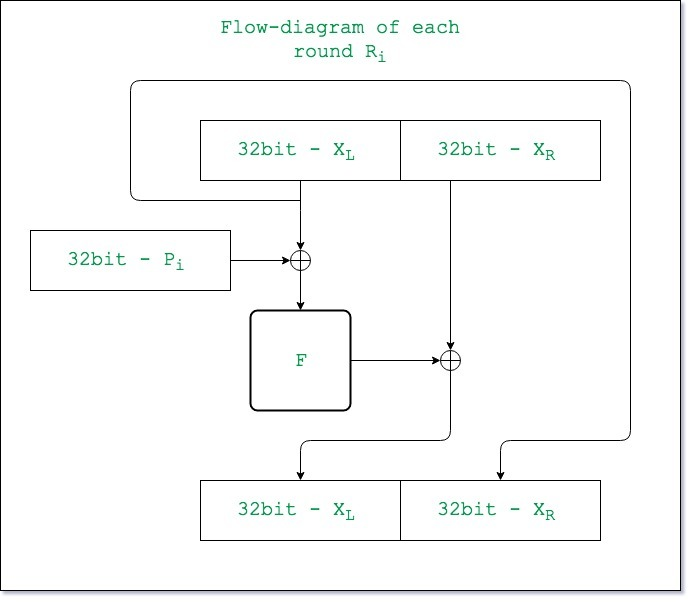
\includegraphics[width=0.9\textwidth]{encription.jpg}
			\caption{grafico che cattura il processo di crittografia dell'algoritmo \cite{blowfish-algorithm}}
			\label{fig:encription}
		\end{figure}


		\section*{Processo di Crittografia e Decrittografia}
		il processo principale di crittografia e decrittografia di Blowfish sta tutto 
		nella funzione \texttt{f} che utilizza le S-box per creare una funzione non
		lineare che contribuisce alla sicurezza dell'algoritmo.

		\begin{figure}[H]
			\centering
			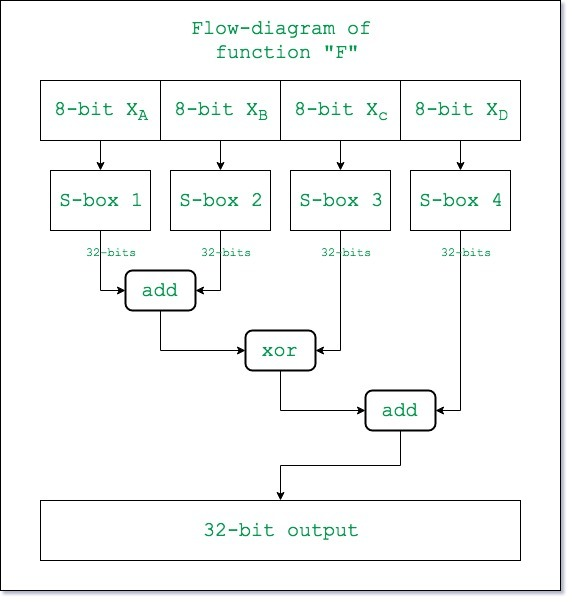
\includegraphics[width=0.9\textwidth]{F-blowfish.jpg}
			\caption{metodo f dell'algoritmo \cite{blowfish-algorithm}}
			\label{fig:f}
		\end{figure}
		% \begin{enumerate}
		% 	\item \textbf{Generazione delle S-Box :} Queste strutture
		% 	vengono inizializzate basandosi sulla chiave fornita dall'utente.
		% 	\item \textbf{Crittografia:} Il testo in chiaro viene diviso in blocchi
		% 	da 64 bit e ogni blocco viene processato attraverso le S-box
		% 	per produrre il testo cifrato.
		% 	\item \textbf{Decrittografia:} Avviene utilizzando la stessa chiave e
		% 	segue un processo simile alla crittografia, ma applicato in ordine
		% 	inverso.
		% \end{enumerate}
		\section*{Funzione $F$ dell'algoritmo Blowfish}

		La funzione $F$ prende in input un valore di 32 bit $x$ e restituisce un valore
		di 32 bit. Essa viene definita come segue:

		\[
			F(x) = ((S_1[a] + S_2[b] \bmod 2^{32}) \oplus S_3[c]) + S_4[d] \bmod 2^{32}
		\]
		\begin{itemize}
			\item $S_1, S_2, S_3, S_4$ sono le S-box dell'algoritmo.
			\item $a$ byte più significativo di x.
			\item $b$ = secondo byte più significativo di x
			\item $c$ = secondo byte meno significativo di x
			\item $d$ = byte meno significativo di x
			
		\end{itemize}
		
		\begin{lstlisting}[style=pseudocode]
			function F(x):
				result = ((S1[a] + S2[b] mod 2^32) xor S3[c]) + S4[d] mod 2^32
				
				return result
		\end{lstlisting}
		\section*{conclusioni sul funzionamento di Blowfish}
		in pratica l'algoritmo di crittografia Blowfish si differenzia
		principalmente dal DES visto a lezione per la sua chiave variabile fino a
		448 bit. \cite{blfh-lenth-key}

		\section*{L'obsolescenza di Blowfish nella prima versione di
		\textit{Password Safe}}
			Uno dei principali punti deboli di Blowfish risiede nella sua
			progettazione con una rete di Feistel di 16 round descritta nei
			paragrafi precedenti. Sebbene non vi siano attacchi pratici noti che
			possano rompere Blowfish con meno di 16 round, la struttura fissa e il
			numero limitato di round non garantiscono la stessa sicurezza di
			algoritmi più moderni come l'AES (Advanced Encryption Standard), che
			offre una configurazione più robusta e una gestione più sicura delle
			chiavi. Inoltre, la progettazione di Blowfish non è ottimizzata per le
			implementazioni hardware moderne, risultando vulnerabile a tecniche come
			gli attacchi \textit{time-memory trade-off} (TMTO) \footnote{Per
			maggiori informazioni sugli attacchi TMTO, si può consultare il seguente
			\href{https://en.wikipedia.org/wiki/Time/Memory/Data_Tradeoff_attack}{link}} e
			l'utilizzo di tabelle precomputate.\\ 
			Con il tempo, la crittografia è diventata un campo in continua 
			evoluzione, con attacchi sempre più sofisticati come quelli
			differenziali e lineari. Mentre Blowfish non è stato completamente
			compromesso da tali attacchi, la sua mancanza di aggiornamenti e
			adattamenti alle nuove minacce lo rende meno preferibile rispetto ad
			altri algoritmi che hanno subito una revisione continua e miglioramenti.\\\\
			Inoltre, il supporto per chiavi di lunghezza fino a 448 bit, sebbene
			teoricamente sufficiente, non offre le stesse garanzie di sicurezza di
			AES con chiavi di lunghezza 256 bit, che è considerato lo standard di
			sicurezza per molte applicazioni critiche. La differenza non è solo
			nella lunghezza delle chiavi, ma anche nella resistenza agli attacchi,
			nella velocità di cifratura e nella versatilità in diversi ambienti
			hardware.e l'utilizzo di tabelle precomputate.\\\\
			Un'altra considerazione critica riguarda la derivazione delle chiavi. La prima
			versione di \textit{Password Safe} potrebbe non aver implementato meccanismi di
			derivazione delle chiavi robusti, come PBKDF2, bcrypt o Argon2, che sono
			progettati per resistere agli attacchi a forza bruta implementando salting e
			iterazioni multiple. Questo rende particolarmente problematico l'uso di Blowfish
			in contesti moderni, dove la sicurezza a lungo termine è essenziale.\\
			\section*{implementazione completa di Blowfish}
			utilizzando la funzione \texttt{F} e le S-box, possiamo scrivere un
			pseudocodice che rappresenta l'intero processo di crittografia e
			decrittografia di Blowfish.
			\begin{lstlisting}[style=pseudocode]
				function encrypt_block(block, key):
					initialize_S_boxes(key)
					left = block[0:32]
					right = block[32:64]
					for i = 1 to 16:
						temp = left
						left = right
						right = temp xor F(right) xor P[i]
					temp = left
					left = right
					right = temp
					return left || right
			\end{lstlisting}
			dove \texttt{P} è un array di 18 elementi che contiene i valori delle chiavi
			derivate dalla chiave principale dell'utente.\\
	\chapter{Bitwarden}
		\section{Introduzione}
		Bitwarden è un password manager open source che offre una soluzione sicura
		per memorizzare e gestire le password.\\ È disponibile su diverse piattaforme,
		tra cui desktop, web, mobile e browser. Bitwarden offre funzionalità di
		sincronizzazione, condivisione e generazione di password, nonché un'interfaccia
		intuitiva e facile da usare.\\
		
		\begin{figure}[H]
			\centering
			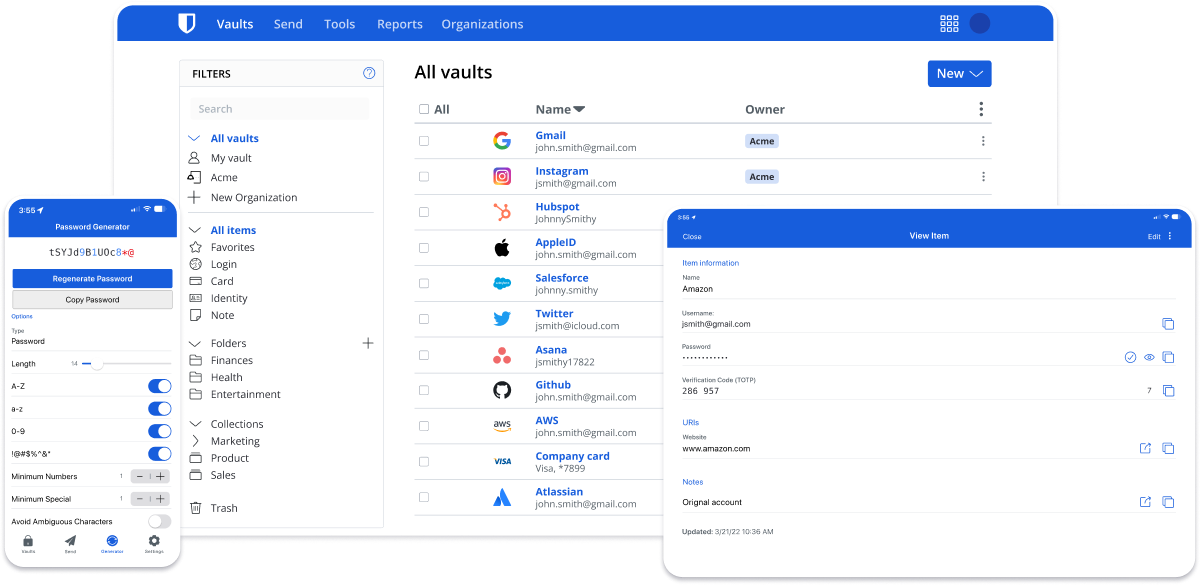
\includegraphics[width=0.9\textwidth]{wardenEnviroment.png}
			\caption{l'enviroment di Bitwarden}
			\label{fig:eviroment}
		\end{figure}

		\section{missione del progetto}
		Bitwarden si pone l'obiettivo di fornire
		una soluzione sicura e affidabile per la gestione delle password.\\ La
		missione di Bitwarden è quella di proteggere la privacy e la sicurezza
		degli utenti, offrendo un servizio gratuito e open source che garantisce
		la riservatezza dei dati e la sicurezza delle informazioni personali.
		Rendendo il suo codice \href{https://github.com/bitwarden}{sorgente}
		pubblico nel 2016, Bitwarden ha dimostrato il suo impegno per la
		trasparenza e la sicurezza, consentendo agli utenti di verificare la
		qualità del software e la sicurezza delle loro password.\\
		
		Come \textit{password safe}, Bitwarden utilizza la master password
		dell'utente per crittografare e proteggere le password memorizzate,
		garantendo che solo l'utente possa accedere ai propri dati. Ma la domanda
		a cui vogliamo rispondere con questa ricerca è: come un software moderno
		opera in un mondo informatico multi device garantendo la massima sicurezza
		quindi sia in locale ma anche in cloud?
	\chapter{Registrazione di un utente su Bitwarden}

		Il processo di hashing della master password in un sistema di gestione
		delle password come Bitwarden segue diversi step che servono a generare 
		una chiave derivata sicura per proteggere le password memorizzate. Questo
		processo permette di non rendere noto il valore della master password
		nemmeno al server storage di Bitwarden.\cite{login-encryption}\\
		Le fasi più critiche e fondamentali verranno prese in esame inseguito.
		\section{generazione della Master Key}
		
		La master password dell'utente viene utilizzata per generare una chiave
		segreta, chiamata \textit{master key}, che verrà utilizzata per cifrare
		e decifrare i dati memorizzati. La master key viene derivata dalla
		combinazione della password principale dell'utente e dell'indirizzo
		email tramite la funzione di derivazione delle chiavi PBKDF2. Questo
		processo utilizza 600.000 iterazioni di HMAC-SHA256, producendo una
		chiave di 256 bit.\\
		\begin{lstlisting}[style=pseudocode]
			function generate_master_key(password, email):
				derived_key = PBKDF2(password, email, 600000, 256)
				master_key = derived_key[0:32]
				
				return master_key
		\end{lstlisting}
		\subsection{la funzione PBKDF2}
			PBKDF2 (Password-Based Key Derivation Function 2) è un meccanismo di
			derivazione di chiavi basato su password ampiamente utilizzato per
			aumentare la sicurezza delle password memorizzate. Il processo inizia
			con l'aggiunta di un "sale", tipicamente una stringa casuale, alla
			password dell'utente. Questo aiuta a proteggere contro gli attacchi di
			dizionario e rainbow table, rendendo ogni hash unico anche se la
			password originale è comune. Successivamente, il valore combinato di
			password e sale viene passato attraverso un algoritmo di hash
			crittografico, in questo caso \textit{HMAC-SHA-256}. HMAC sta per Hash-based
			Message Authentication Code, che è un tipo di funzione di hash che
			fornisce sia l'integrità dei dati che l'autenticazione del messaggio.
			SHA-256 è parte della famiglia di algoritmi Secure Hash Algorithm e
			produce un hash di lunghezza fissa di 256 bit.\cite{PBKDF2}\\\\
			Dopo il primo hashing, il valore ottenuto viene nuovamente salato e hashato
			molteplici volte. Il numero di iterazioni, \textit{streaching-function}\cite{PBKDF2-streaching-function}, è
			configurabile e serve a rendere il processo di derivazione della chiave
			intenzionalmente lento. Questo rallentamento è critico per la sicurezza, poiché
			rende gli attacchi di forza bruta e di ricerca esaustiva molto più dispendiosi
			in termini di tempo e risorse computazionali. Con ogni iterazione, l'hash
			diventa più resistente agli attacchi, aumentando così la sicurezza della chiave
			derivata.\\\\
			La chiave finale ottenuta dopo l'ultima iterazione è la chiave principale, che
			non è altro che un altro hash che sarà utilizzato per ulteriori operazioni
			crittografiche, come l'hash della password principale. Quest'ultimo è il valore
			che viene effettivamente utilizzato per verificare l'identità dell'utente
			durante il processo di autenticazione. Ogni volta che l'utente inserisce la sua
			password, il sistema ripete il processo di derivazione della chiave e confronta
			l'hash risultante con quello memorizzato. Se corrispondono, l'accesso è
			concesso.
			\begin{lstlisting}[style=pseudocode]
				function PBKDF2(password, salt, iterations, key_length):
					key = password
					for i = 1 to iterations:
						key = HMAC-SHA256(key, salt)
					return key[0:key_length]
			\end{lstlisting}
		\subsection{HMAC-SHA-256}
			mentre a lezione abbiamo studiato e visto il funzionamento di SHA-256, mi sento 
			di approfondire il funzionamento di HMAC-SHA-256.\\
			HMAC sta per Hash-based Message Authentication Code, in questo caso specifico
			la funzione di hash scelta è quella vista a lezione, ora vediamo come la opera 
			per rendere sicura l'informazione.\cite{HMAC}
			\begin{figure}[H]
				\centering
				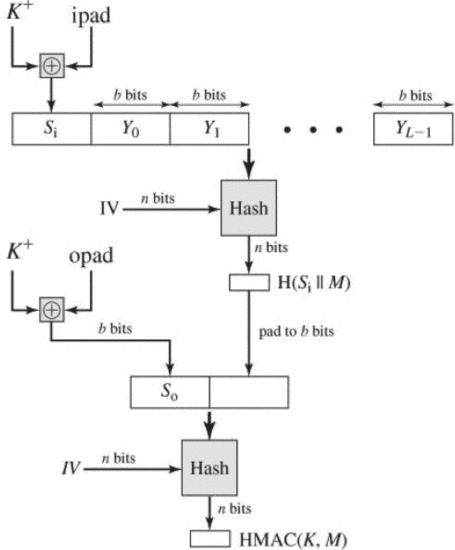
\includegraphics[width=0.8\textwidth]{HMAC-structure.png}
				\caption{funzionamento di HMAC-SHA-256}
				\label{fig:hmac-sha256}
			\end{figure}
			\begin{enumerate}
				\item Aggiungere zeri all'inizio di K per creare una stringa di bit $b$
				chiamata $K^+$.
				\item Fare lo XOR tra $K^+$ e \textit{ipad} per produrre il blocco di bit
				$b$ $S_i$.
				\item Aggiungere $M$ a $S_i$.
				\item Applicare l'algoritmo di hash $H$ al flusso generato nel passaggio 3.
				\item Fare lo XOR tra $K^+$ e \textit{opad} per produrre il blocco di bit
				$b$ $S_0$.
				\item Aggiungere il risultato dell'hash del passaggio 4 a $S_0$.
				\item Applicare l'algoritmo di hash $H$ al flusso generato nel passaggio 6 e
				produrre il risultato finale.
			\end{enumerate}

		\section{Stretched Master Key}
		La master key risultante viene
		ulteriormente elaborata tramite l'algoritmo HKDF con SHA-256, che include una
		fase di espansione delle chiavi, per produrre una chiave estesa di 512 bit.
		Questa chiave estesa è utilizzata per cifrare i dati memorizzati nella
		cassaforte digitale dell'utente, compresi i vari segreti e le chiavi di
		cifratura.
		\begin{lstlisting}[style=pseudocode]
			function stretch_master_key(master_key):
				stretched_key = HKDF(master_key, 512)

				return stretched_key
		\end{lstlisting}
		\subsection{HKDF}
			HKDF (HMAC-based Key Derivation Function) è un algoritmo di derivazione delle
			chiavi basato su HMAC che consente di generare chiavi di lunghezza variabile a
			partire da una chiave segreta. 
			
			HKDF è un meccanismo per derivare chiavi crittografiche sicure da un
			materiale di chiave iniziale (Initial Key Material, IKM). L'algoritmo è
			suddiviso in due fasi principali: estrazione ed espansione.

		\subsection*{Fase 1: Estrazione}

		\textbf{Scopo}: Estrarre una chiave pseudocasuale (PRK) dal materiale di
		chiave iniziale.\\
		\textbf{Procedura}: Si utilizza una funzione HMAC con un hash
		crittografico (ad esempio, SHA-256). Il sale (`salt`) è un valore
		opzionale; se non fornito, si usa una stringa di zeri della lunghezza
		dell'hash\cite{HMAC-expand}.

		\[
		\text{PRK} = \text{HMAC}_\text{hash}(\text{salt}, \text{IKM})
		\]

		\subsection*{Fase 2: Espansione}

		\textbf{Scopo}: Derivare una o più chiavi di output (Output Key
		Material, OKM) dalla PRK.\\
		\textbf{Procedura}: Utilizzando nuovamente HMAC, la PRK è impiegata come
		chiave per l'HMAC e un contesto (`info`) come input. L'output è una
		concatenazione di più blocchi HMAC. \cite{HMAC-expand}

		\[
		T(0) = \emptyset
		\]

		\[
		T(1) = \text{HMAC}_\text{hash}(\text{PRK}, T(0) \| \text{info} \| 0x01)
		\]

		\[
		T(2) = \text{HMAC}_\text{hash}(\text{PRK}, T(1) \| \text{info} \| 0x02)
		\]

		\[
		\ldots
		\]

		\[
		T(n) = \text{HMAC}_\text{hash}(\text{PRK}, T(n-1) \| \text{info} \| n)
		\]

		\[
		\text{OKM} = T(1) \| T(2) \| \ldots \| T(n)
		\]

		\textbf{Dove}:
		\begin{itemize}
			\item \(\| \) denota la concatenazione.
			\item \( n \) è il numero di blocchi necessari per ottenere la
			lunghezza desiderata dell'OKM.
		\end{itemize}

		\subsection*{Caratteristiche Principali}
		\begin{itemize}
			\item \textbf{Sicurezza}: HKDF è progettato per essere resistente a
			vari attacchi, mantenendo segrete le chiavi derivate anche se una di
			esse viene compromessa.
			\item \textbf{Modularità}: Può utilizzare diverse funzioni hash,
			adattandosi a diverse esigenze di sicurezza.
			\item \textbf{Efficienza}: È efficiente in termini computazionali e
			di memoria.
		\end{itemize}

		Questo processo garantisce che anche se due utenti hanno la stessa master password, i valori hash memorizzati saranno diversi grazie all'uso del salt. Inoltre, l'uso di PBKDF2 rende l'attacco di forza bruta molto più difficile.
		ecco lo pseudocode completo dell'operazione:
		\begin{lstlisting}[style=pseudocode]
			function hash_master_password(password, salt):
				input = password || salt
				hash = SHA-256(input)
				derived_key = PBKDF2(hash, salt, iterations, key_length)
				stored_value = {salt, derived_key}
				
				return stored_value
		\end{lstlisting}
		\subsection{PBKDF2 o Argon2?}
		Dalla versione 2023.2.0 di Bitwarden, è stata inserita la possibilità
		di scegliere tra PBKDF2 e Argon2 come algoritmo di derivazione delle
		chiavi per l'hashing della master password. Argon2 è un algoritmo di
		derivazione delle chiavi. Vincitore del concorso Password Hashing
		Competition (PHC) nel 2015. Vediamo come si comporta e che differenze 
		ha rispetto a PBKDF2.\\
		La differenza fra PBKDF2 e Argon2 sta nel fatto che Argon2 sfrutta
		una memoria più grande e un tempo di esecuzione più lungo, grazie alla
		sua funzione principale di stretching. 
		\subsection*{fase di espanzione di Argon2}
		una volta presa una stringa da criptare, Argon2 si comporta nel seguente modo:
		\begin{enumerate}
			\item Viene generato un blocco di memoria di dimensione fissa, chiamato
			\textit{lanes}, che contiene il materiale di chiave iniziale (IKM).
			\item Il blocco di memoria viene diviso in segmenti di dimensione fissa,
			chiamati \textit{lanes}.
			\item Ogni segmento viene elaborato in parallelo, utilizzando una funzione
			di hash crittografico (ad esempio, SHA-256).
			\item I risultati di ogni segmento vengono combinati per produrre un'unica
			chiave di output.
		\end{enumerate}
		\section*{Funzione di compressione G e funzione di round P di Blake2b}

			La funzione di compressione \textbf{G} è costruita sulla funzione di
			round \textbf{P} di \textbf{Blake2b}. La funzione \textbf{P} opera su un
			input di 128 byte, che può essere visto come 8 registri di 16 byte:\cite{argon2}
			\[
			P(A_0, A_1, \dots, A_7) = (B_0, B_1, \dots, B_7).
			\]
			La funzione di compressione \textbf{G(X, Y)} opera su due blocchi di
			1024 byte, \textbf{X} e \textbf{Y}. Inizialmente, si calcola:
			\[
			R = X \oplus Y.
			\]

			Quindi, \textbf{R} è visto come una matrice 88 di registri di 16 byte.
			La funzione \textbf{P} viene applicata prima per riga e poi per colonna
			per ottenere \textbf{Z}:

			\[
			(Q_0, Q_1, \dots, Q_7) \leftarrow P(R_0, R_1, \dots, R_7);
			\]

			\[
			(Q_8, Q_9, \dots, Q_{15}) \leftarrow P(R_8, R_9, \dots, R_{15});
			\]

			\[
			\ldots
			\]

			\[
			(Q_{56}, Q_{57}, \dots, Q_{63}) \leftarrow P(R_{56}, R_{57}, \dots, R_{63});
			\]

			\[
			(Z_0, Z_8, Z_{16}, \dots, Z_{56}) \leftarrow P(Q_0, Q_8, Q_{16}, \dots, Q_{56});
			\]

			\[
			(Z_1, Z_9, Z_{17}, \dots, Z_{57}) \leftarrow P(Q_1, Q_9, Q_{17}, \dots, Q_{57});
			\]

			\[
			\ldots
			\]

			\[
			(Z_7, Z_{15}, Z_{23}, \dots, Z_{63}) \leftarrow P(Q_7, Q_{15}, Q_{23}, \dots, Q_{63}).
			\]

			Infine, \textbf{G} produce l'output \textbf{Z $\oplus$ R}:

			\[
			G : (X, Y) \rightarrow R = X \oplus Y \rightarrow P \rightarrow Q \rightarrow P \rightarrow Z \rightarrow Z \oplus R.
			\]
			
			\section*{Perché "Decompressione"?}
			
			Il termine "decompressione" si riferisce al processo attraverso il
			quale un'informazione sintetizzata o combinata (come nel caso di \(
			R = X \oplus Y \)) viene espansa in una rappresentazione più
			articolata attraverso vari passaggi di trasformazione. In
			particolare, la funzione \( P \) applicata row-wise e column-wise
			agisce in modo da rimescolare e ridistribuire l'informazione
			contenuta in \( R \), aumentando così la sua entropia e rendendo
			l'output meno riconoscibile rispetto agli input originali.
			
			Questo processo di "decompressione" assicura che, sebbene il
			risultato finale (output di \( G \)) sia complesso e diffuso, esso
			conserva una relazione matematica precisa con i dati di input.
		
			\section{utilizzo delle due Master Key}
			Insomma, tutta questa fatica per avere due chiavi fortemente sicure,
			ma a cosa servono?\\
			Possiamo dire che siamo a questo punto dello schema crittografico di Bitwarden:
			\begin{figure}[H]
				\centering
				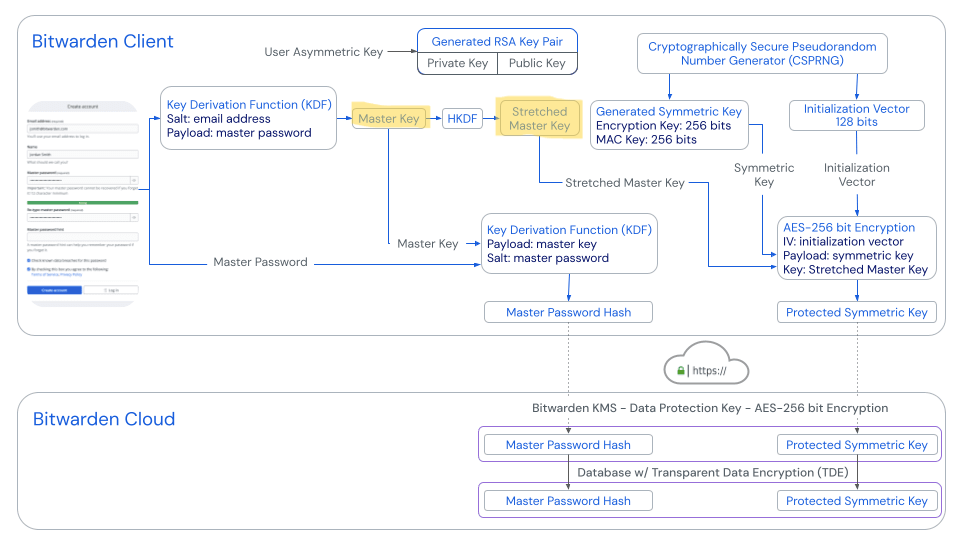
\includegraphics[width=0.9\textwidth]{masterKeyGenerated.png}
				\caption{fasi di generazione delle chiavi}
				\label{fig:masterKey}
			\end{figure}
			La Master Password quindi viene solo utilizzata per generare una complessa
			"danza" crittografica. In questo modo non viene mai salvata in chiaro 
			se non nell'istante in cui il client la inserisce.\\
			Ora vediamo come Bitwarden ha deciso come utilizzare queste due chiavi
			per poter riconoscere l'utente garantendone la massima sicurezza.
			\subsection{Master Password Hash}
			 Viene generata utilizzando un algoritmo di derivazione della chiave, 
			 abbiamo già visto come funziona PBKDF2, una volta fatto il primo accesso
			 puoi decidere quale algoritmo utilizzare fra quelli precedentemente presentati
			\subsection{Protected Symmetric Key}
				generata con un algoritmo AES-256 che ora spieghiamo nel dettaglio:\\
				L'AES-256 (Advanced Encryption Standard con una chiave di 256
				bit)\\ è un algoritmo di cifratura a blocchi che utilizza una chiave
				simmetrica per cifrare e decifrare i dati.
				\newpage
				\subsection{Come applica Confusine AES-256? }
				\subsection*{SubBytes e S-Box}

				\begin{itemize}
					\item \textbf{S-Box (Substitution Box)}: L'S-Box è una tabella
					di sostituzione che mappa ogni byte del blocco di stato a un
					altro byte. Questa mappatura non è lineare, il che significa che
					piccoli cambiamenti nel testo in chiaro o nella chiave possono
					causare cambiamenti significativi nel testo cifrato. L'S-Box di
					AES è progettata per resistere ad attacchi di crittoanalisi
					differenziale e lineare.
					\item \textbf{SubBytes}: In questa operazione, ogni byte del
					blocco di stato (una matrice 4·4 di byte) viene sostituito con
					il byte corrispondente nell'S-Box. Questa operazione introduce
					confusione, in quanto la sostituzione non segue un modello
					prevedibile e aumenta la complessità dell'analisi del testo
					cifrato.
					\begin{figure}[H]
						\centering
						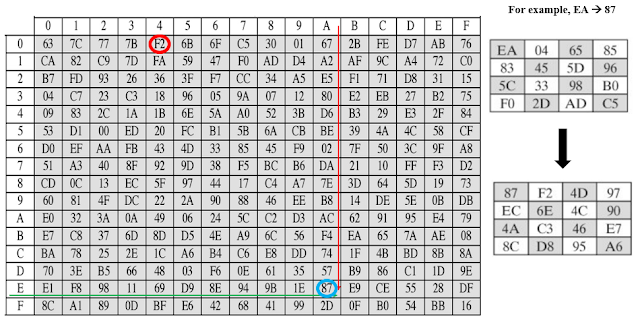
\includegraphics[width=1.1\textwidth]{sbox.png}
						\caption{spostamento sulla matrice 16·15 di S-Box, nelle varianti con meno bit di AES si utilizzano matrici più piccole}
					\end{figure}
					
				\end{itemize}
				\newpage
				\subsection{come applica Diffusione?}
				\subsection*{ShiftRows}

				\begin{itemize}
				\item \textbf{ShiftRows} è un'operazione in cui i byte nelle
				righe della matrice di stato sono ciclicamente spostati a
				sinistra. La prima riga rimane inalterata, la seconda riga è
				spostata di una posizione, la terza di due posizioni e la quarta
				di tre posizioni. Questo spostamento crea una diffusione tra i
				byte nelle diverse colonne della matrice.
				\begin{figure}[H]
					\centering
					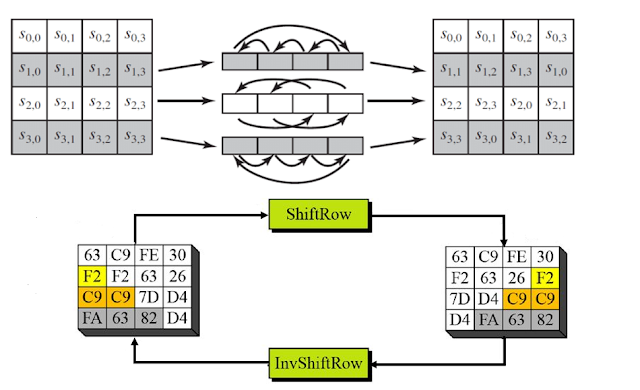
\includegraphics[width=0.9\textwidth]{shiftRow.png}
					\caption{rappresentazione matriciale di SubBytes}
				\end{figure}
				\end{itemize}

				\subsection*{MixColumns}

				\begin{itemize}
				\item è un'operazione che applica una
				trasformazione lineare ai byte di ogni colonna della matrice di
				stato. Ogni colonna è trattata come un vettore di quattro byte e
				viene moltiplicata, in un campo di Galois (matematica finita),
				per una matrice fissa, che è invertibile. Questa operazione
				mescola i byte all'interno di ciascuna colonna, assicurando che
				i cambiamenti in un singolo byte si diffondano a tutti gli altri
				byte della colonna.
				\end{itemize}
				\newpage
				\subsection*{AddRoundKey}
				Anche se l'operazione di \textbf{AddRoundKey} non contribuisce
				direttamente alla confusione e alla diffusione, è essenziale per
				la sicurezza dell'algoritmo. In questa fase, una chiave di round
				derivata dalla chiave principale viene aggiunta al blocco di
				stato tramite l'operazione di XOR. Ogni round ha una chiave
				diversa, derivata attraverso un processo noto come "expansion
				key". Questa aggiunta introduce un nuovo livello di sicurezza,
				rendendo ogni round unico.
				\begin{figure}[H]
					\centering
					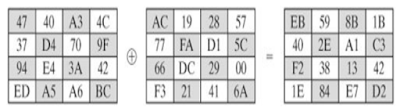
\includegraphics[width=0.9\textwidth]{roundKey.png}
					\caption{rappresentazione matriciale di round key}
				\end{figure}
							
			\chapter{accesso di Bob}
				\textbf{Contesto}: Bob è un utente di Bitwarden e vuole accedere al suo account utilizzando la sua \textit{email} e la sua \textit{master password}.

				\subsection*{Passaggi dell'accesso di Bob}

				\begin{enumerate}
					\item \textbf{Inserimento delle Credenziali}:
					\begin{itemize}
						\item \textit{Email}: Bob inserisce il suo indirizzo email, ad esempio, \texttt{bob@example.com}.
						\item \textit{Master Password}: Bob inserisce la sua master password.
					\end{itemize}
					
					\item \textbf{Derivazione della Master Key}:
					\begin{itemize}
						\item Localmente sul dispositivo di Bob, la master password viene combinata con la sua email (\texttt{bob@example.com}) come sale in un processo di derivazione della chiave utilizzando \textbf{PBKDF2} con un numero elevato di iterazioni (ad esempio, 600.000). Questo produce una chiave di 256 bit chiamata \textbf{Master Key}.
					\end{itemize}

					\item \textbf{Creazione dell'Hash della Master Password}:
					\begin{itemize}
						\item La Master Key viene usata per generare un hash della master password (MPH). Questo hash è derivato usando \textbf{PBKDF-SHA256} con un payload della Master Key e un \texttt{salt} derivato dalla master password. Questo hash viene inviato ai server di Bitwarden per l'autenticazione.
					\end{itemize}

					\item \textbf{Autenticazione sul Server}:
					\begin{itemize}
						\item I server di Bitwarden confrontano l'hash inviato con l'hash memorizzato corrispondente. Se gli hash corrispondono, l'autenticazione è considerata valida.
					\end{itemize}

					\item \textbf{Decriptazione della Protected Symmetric Key}:
					\begin{itemize}
						\item Sul dispositivo di Bob, la \textbf{Stretched Master Key} viene derivata dalla Master Key utilizzando l'\textbf{HKDF} (HMAC-based Extract-and-Expand Key Derivation Function).
						\item La Stretched Master Key viene quindi utilizzata per decriptare la \textbf{Protected Symmetric Key}, che è memorizzata sul server e criptata con la Stretched Master Key. La Protected Symmetric Key decriptata fornisce accesso alla \textbf{User Symmetric Key}, che è la chiave usata per decriptare i dati del vault.
					\end{itemize}

					\item \textbf{Accesso ai Dati}:
					\begin{itemize}
						\item Con la User Symmetric Key, Bob può ora accedere ai dati criptati nel suo vault. Questo processo di decriptazione avviene interamente sul suo dispositivo.
					\end{itemize}
				\end{enumerate}

				\section*{Controesempio: Accesso Fallito}

				Immaginiamo che Bob, accidentalmente, inserisca una master password errata o un'email errata:

				\begin{enumerate}
					\item \textbf{Inserimento delle Credenziali Errate}:
					\begin{itemize}
						\item Bob inserisce una master password o un'email sbagliata.
					\end{itemize}

					\item \textbf{Derivazione della Master Key Errata}:
					\begin{itemize}
						\item L'errore nella master password o nell'email porta alla derivazione di una \textbf{Master Key errata}.
					\end{itemize}

					\item \textbf{Creazione di un Hash della Master Password Errato}:
					\begin{itemize}
						\item La Master Key errata produce un hash della master password che non corrisponde a quello memorizzato sui server di Bitwarden.
					\end{itemize}

					\item \textbf{Autenticazione Fallita}:
					\begin{itemize}
						\item Gli hash non corrispondono, quindi l'autenticazione fallisce. Bob non può accedere al suo account perché il server non autorizza l'accesso.
					\end{itemize}

					\item \textbf{Mancata Decriptazione}:
					\begin{itemize}
						\item Poiché l'autenticazione fallisce, Bob non riceve la \textbf{Protected Symmetric Key} corretta, e quindi non può decriptare i dati del suo vault. Anche se avesse ricevuto una chiave protetta, la Stretched Master Key errata non sarebbe in grado di decriptarla correttamente.
					\end{itemize}
				\end{enumerate}

				Questo processo garantisce che solo chi conosce la master password corretta possa accedere ai dati criptati, proteggendo l'utente da accessi non autorizzati.
			\chapter{Conclusioni}
			Personalmente, Dopo questa ricerca mi sento di dire che Bitwarden è un
			software molto sicuro e affidabile per la gestione delle password.
			Mi piace pensare che la crittografia sia utilizzata per scopi positivi
			e Bitwarden è la migliore offerta open source per la gestione delle
			proprie password.\\
			Ho apprezzato talmente tanto la complessità e la capacità degli ingegneri
			nel saper architettare un meccanismo crittografico e talmente fine da non 
			aver paura di ricervere attacchi nel server cloud, poichè anche se venissero 
			rubati i dati, sarebbero inutilizzabili senza la master password.\\ Per questi 
			motivi e per lo studio fornito sulla complessità crittografica che ho deciso 
			di aprire un accounti Bitwarden per gestire, da qui in poi, i miei account personali \\
			\bibliography{refs}
			\renewcommand{\bibsection}{}
			
	
\end{document}
